\documentclass[11pt]{handout}
\usepackage{moreverb}
\usepackage{tabularx}
\usepackage{epsf}
\usepackage{epsfig}
\usepackage{fancyheadings}
\usepackage{fancybox}

\renewcommand{\coursetitle}{ECE 320}
\renewcommand{\handouttitle}{Symbol Timing Recovery}
\renewcommand{\handoutauthor}{Michael Kramer}
\renewcommand{\semestertitle}{Spring 2001}

\newcommand{\bea}{\begin{eqnarray}}
\newcommand{\eea}{\end{eqnarray}}

\setlength{\parindent}{5mm}
\begin{document}

\setlength{\baselineskip}{0.5cm}
\setlength{\parskip}{0.5cm}

\makeboxtitle
\vspace{0.3cm}

\section{Introduction:}

%AUTHOR: Michael Kramer
This intent of this receiver exercise is to provide an introduction
to the primary components of a digital communications receiver
with specific focus on the symbol timing recovery section.
After the received signal has been coherently demodulated
(carrier recovery will be discussed in the next handout)
and filtered with a low-pass FIR, the next step for the
receiver is to sample the recovered message signals (in-phase
and quadrature channels) at the desired symbol rate.
Although the symbol rate is typically known to the receiver,
what is unknown is when to sample the signal.
Using a feed-back based approach, the objective of the symbol 
timing recovery loop then is to find the best time to sample the 
received signal. 
 

In Figure \ref{fig: receiver}
the transmitted signal is coherently demodulated
with both a sine and cosine then low-pass filtered
to remove the double frequency terms yielding the
recovered in-phase and quadrature signals, $\hat{s}_I(n)$ and
$\hat{s}_Q(n)$.  Both branches are then fed through
a matched filter and re-sampled at the symbol rate.
The matched filter is simply an FIR filter with an
impulse response matched to the transmitted pulse.

\begin{figure}[ht]
   \begin{center}
      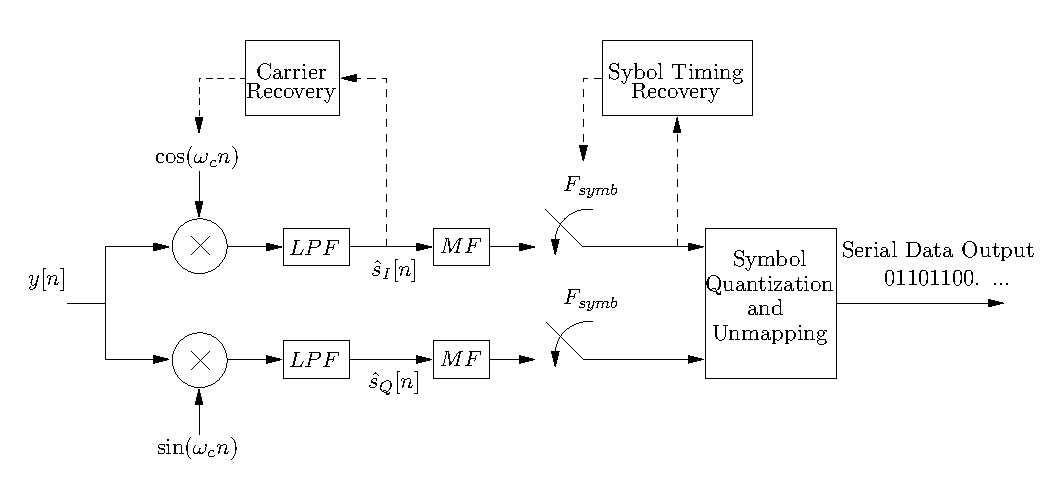
\epsfig{file=receiv.eps,width=15cm}
      \caption{Digital receiver system.}
      \label{fig: receiver}
   \end{center}
\end{figure}

The matched, or averaging filter in the above block diagram is included
both to aid in timing recovery as well as help suppress the effects of noise.  
If we consider the square wave shown in Figure \ref{fig: clean_BPSK} as a 
potential recovered in-phase (or quadrature) signal (i.e. we sent the
data $+1, -1, +1, -1, ...$) then sampling at any point
other than the symbol transitions will result in the correct
data.  
\begin{figure}[ht]
   \begin{center}
      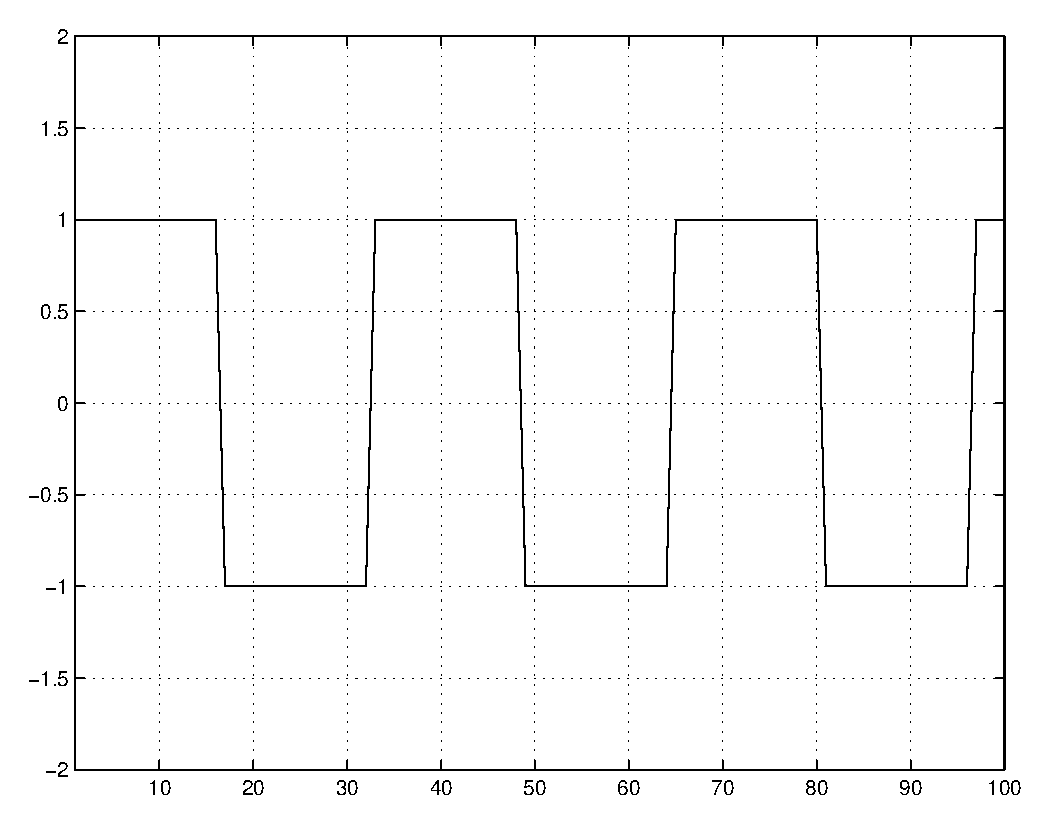
\epsfig{file=clean_bpsk.eps,width=6cm}
      \caption{Clean BPSK waveform.}
      \label{fig: clean_BPSK}
   \end{center}
\end{figure}

However, in the presence of noise, the received waveform looks like
that shown in Figure \ref{fig: noisy_BPSK}
\begin{figure}[ht]
   \begin{center}
      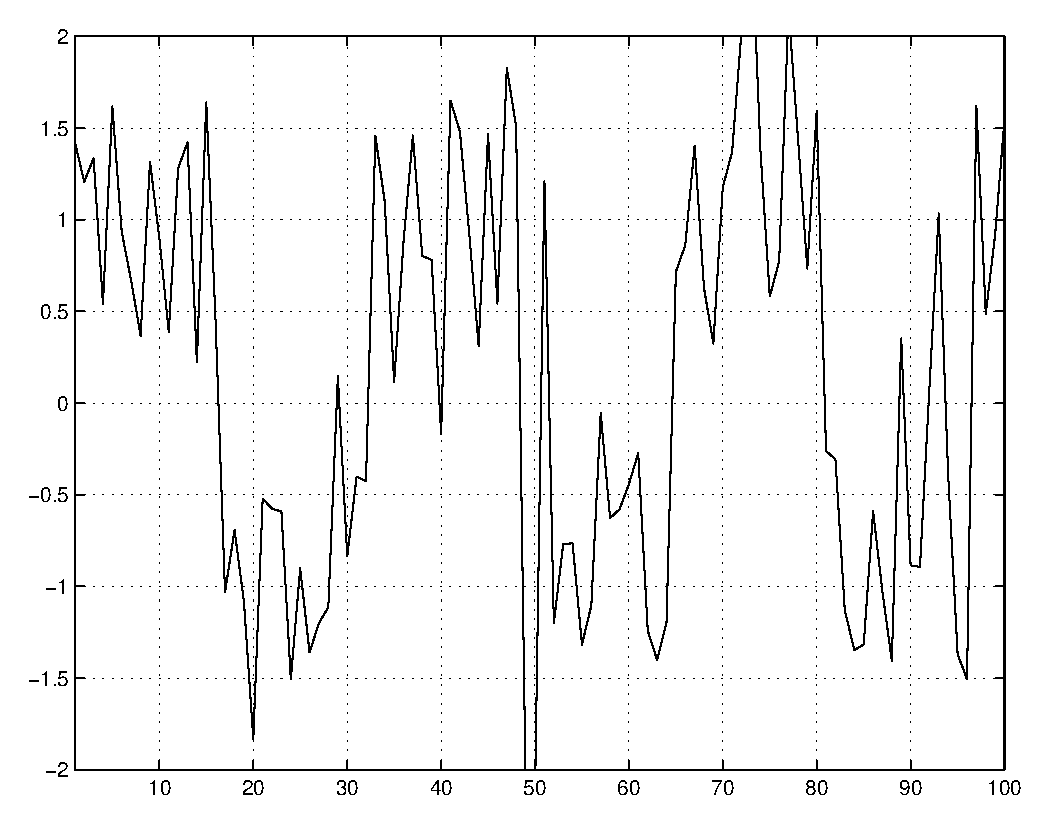
\epsfig{file=noisy_bpsk.eps,width=6cm}
      \caption{Noisy BPSK waveform.}
      \label{fig: noisy_BPSK}
   \end{center}
\end{figure}
and sampling it at any point could result in an incorrect data decision,
for instance if the noise amplitude at the sample taken is greater than
the symbol amplitude.
By taking 
an average over the symbol duration we can obtain a better estimate
of the true data bit being sent; that is, either $+1$ or $-1$.  
This averaging filter can be implemented
using a simple rectangular filter that is the same length as the 
expected symbol period.  
Figures \ref{fig: clean_mf_out} and \ref{fig: noisy_mf_out}
show the result of passing both the clean 
and noisy signal through such an averaging filter.

\begin{figure}[ht]
   \begin{center}
      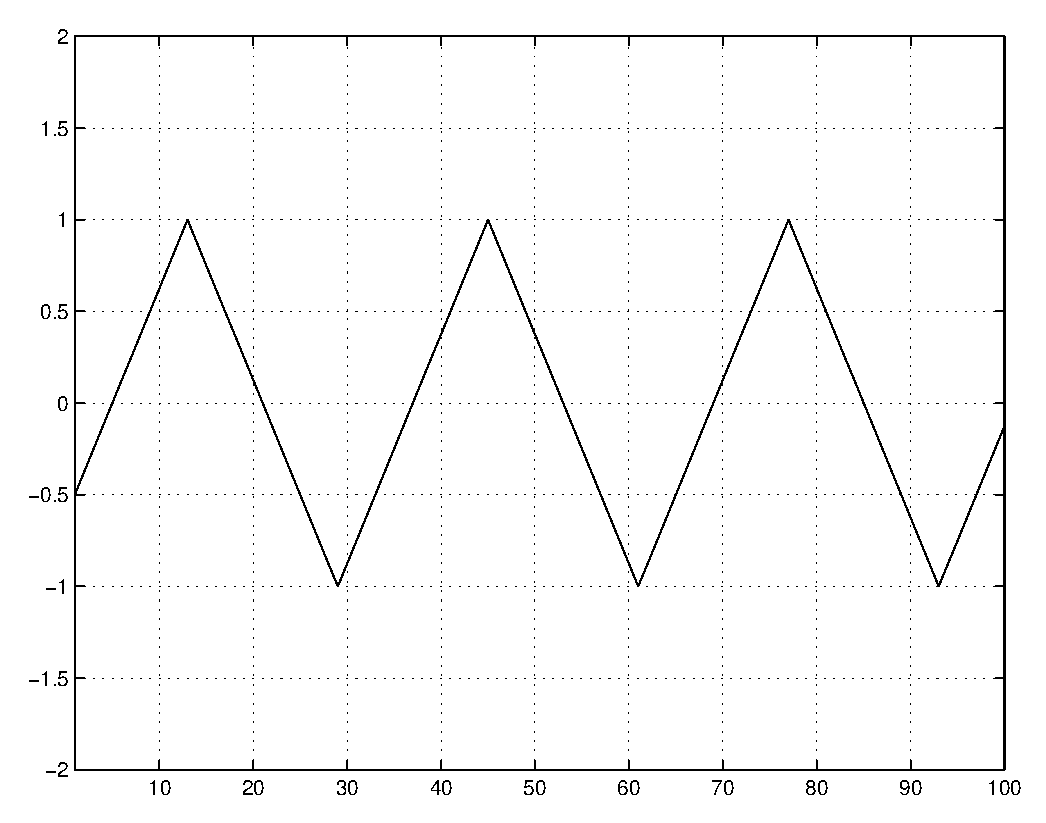
\epsfig{file=clean_mf_out.eps,width=6cm}
      \caption{Clean averaging filter output.}
      \label{fig: clean_mf_out}
   \end{center}
\end{figure}
\begin{figure}[ht]
   \begin{center}
      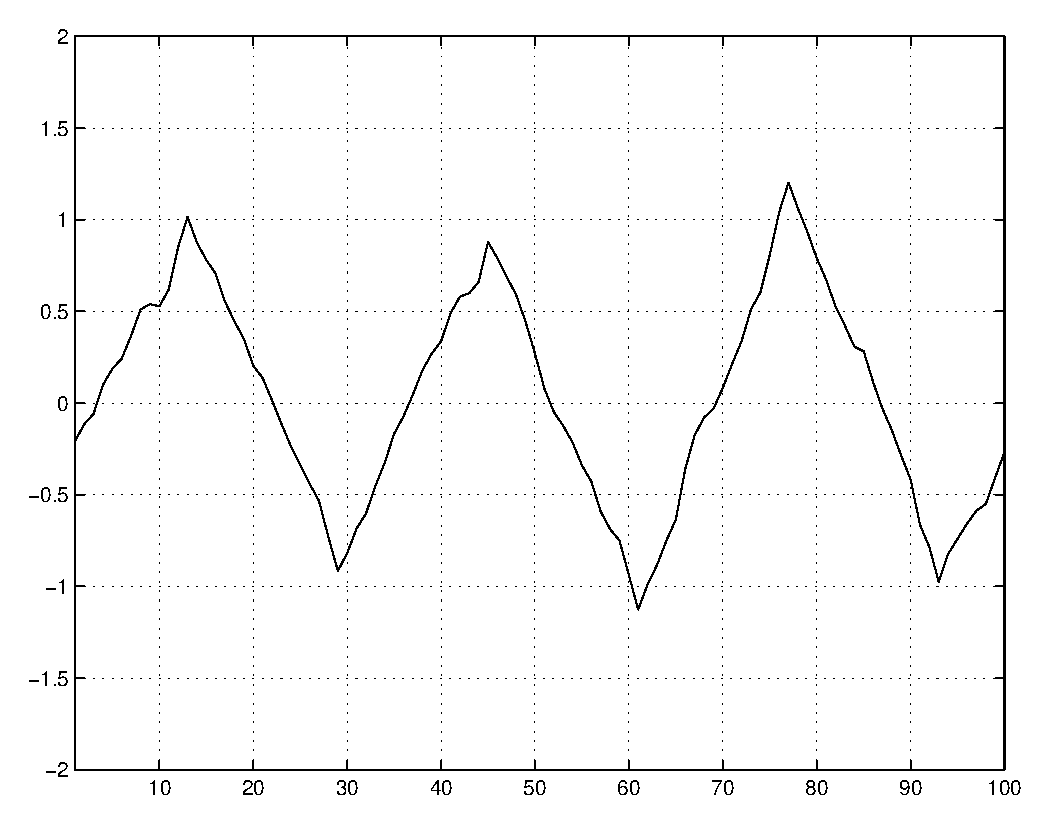
\epsfig{file=noisy_mf_out.eps,width=6cm}
      \caption{Averaging filter output in the presence of noise.}
      \label{fig: noisy_mf_out}
   \end{center}
\end{figure}

Note that in both cases the output of the averaging filter has peaks
where the averaging filter exactly lines up with the symbol, and a positive
(negative) peak indicates that a $+1$ ($-1$) was sent.  Although there still
exists some noise in second figure, the peaks 
are relatively easy to distinguish and yield considerably more
accurate data estimation ($+1$ or $-1$) than we could get
by sampling the original noisy signal in Figure \ref{fig: noisy_BPSK}.
This averaging filter is referred to as a matched filter as it
is matched to the symbols being sent, in this case rectangular
pulses.  For digital communications schemes involving different
symbol sets (frequency shift keying, spread-spectrum, etc.) 
the form of the matched filter will be different.  
Refer to the listed references for more information on symbol timing and 
matched filters for different symbol waveforms.


The remainder of this handout describes a method for designing
a symbol timing recovery loop for a BPSK signal (equivalent to a 
QPSK signal where only the in-phase signal is used).  
As with the above examples,
a symbol period of $T_s = 16$ samples is assumed.  

\paragraph{Early/late sampling:}
One simple method for symbol-timing recovery is performed 
using a delay locked loop (DLL), the block diagram shown  in 
Figure \ref{fig: dll} the necessary components.

\begin{figure}[ht]
   \begin{center}
      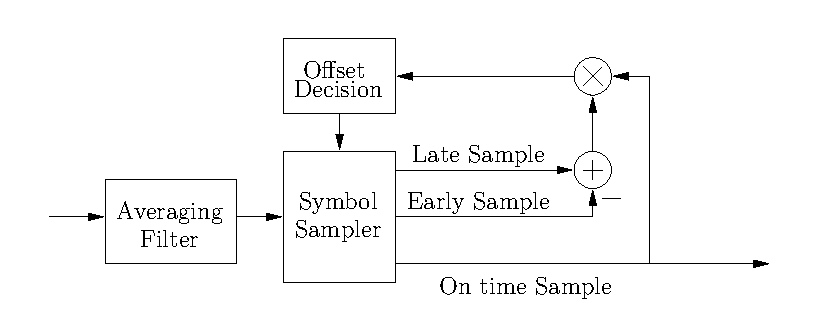
\epsfig{file=dll.eps,width=9cm}
      \caption{DLL block diagram.}
      \label{fig: dll}
   \end{center}
\end{figure}

Consider the sawtooth waveform shown in Figure (the output of the
averaging filter with a square wave as input). If the symbol sampling 
phase is correct, we will sample this wave right at the peak,
otherwise we will either be sampling too early or too
late.  Figure \ref{fig: on-time_ex} shows an example
of proper sampling phase, notice that the on-time
sample is at the peak.

\begin{figure}[ht]
   \begin{center}
      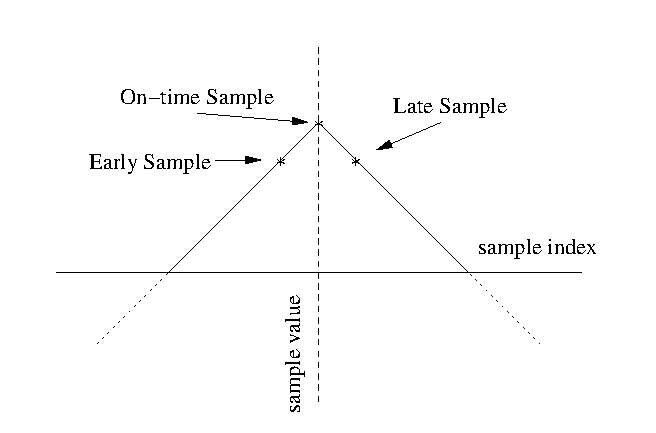
\epsfig{file=ontime.eps,width=8cm}
      \caption{Matched sampling example.}
      \label{fig: on-time_ex}
   \end{center}
\end{figure}

Figures \ref{fig: early_ex} and \ref{fig: late_ex}
show examples of early and late sampling respectively.

\begin{figure}[ht]
   \begin{center}
      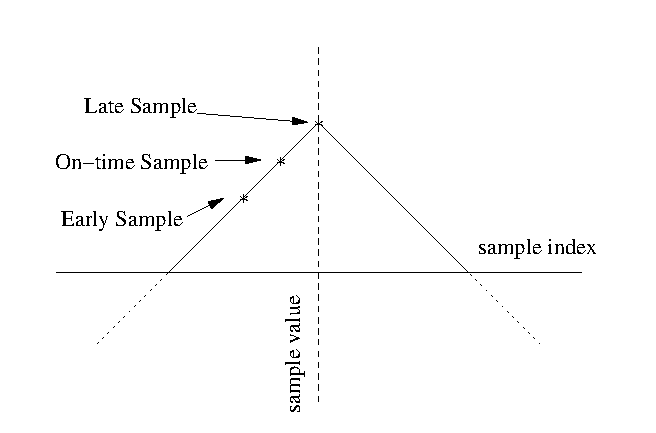
\epsfig{file=early.eps,width=8cm}
      \caption{Early sampling example.}
      \label{fig: early_ex}
   \end{center}
\end{figure}

\begin{figure}[ht]
   \begin{center}
      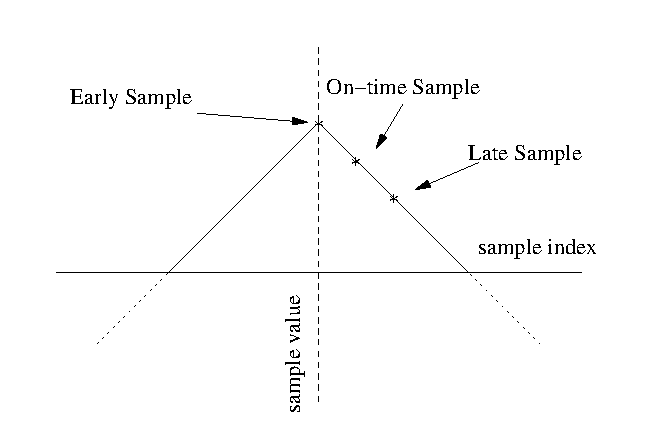
\epsfig{file=late.eps,width=8cm}
      \caption{Late sampling example.}
      \label{fig: late_ex}
   \end{center}
\end{figure}

Note that in the early sampling case, the input to the decision
maker is positive (late - early $>$ 0) and negative for the late
sampling scenario.  The (late - early) value is multiplied
by the on-time value in case that the peak of the sawtooth
wave is negative.  This will ensure that the input to the
decision offset block has the correct sign regardless of whether
the peak is positive or negative.

\paragraph{Sampling counter:}

The symbol sampler keeps track of its own counter, when the
counter reaches zero the averaging filter output is sampled
yielding the on-time sample and the counter is reset to $T_s$
samples.  It is the responsibility of the decision offset block
to adjust this counter and either increment or decrement it
depending on whether the on-time samples are considered early
or late.

The decision offset block maintains an early/late accumulator
that keeps a running total of the decision statistic (on-time $\times$
[ late - early ] ). When this value exceeds some
threshold the counter is adjusted.
If we are sampling too early, the early/late accumulator will get lager
and when it exceeds the threshold point, we adjust the
counter to $(T+1)$ and clear out the accumulated decision
statistic.  This will result in shifting the sampling point
towards the desired early sample.  If the decision
statistic goes below the negative of the threshold, then
the counter is set to $(T-1)$ and the accumulated decision
statistic is cleared.
The reason for accumulating the results of several sampling
periods before adjusting the sampling counter is to keep
the adjustment from being to jittery, as well as to help
filter out any noise.


\section{Matlab Simulation}

%AUTHOR:Michael Kramer
Because the symbol-timing requires a feed-back loop, you will
have to simulate the DLL on a sample by sample basis in \matlab.

Using an square wave of period $32$ samples as input, simulate
the DLL system shown in Figure \ref{fig: dll}.  Your input
should be several hundred periods long and you will want to
set the early/late accumulations threshold to $1.0$ to start with 
(How will a different threshold level affect the locking ability of the DLL?)

The figures below show the matched filter output and the corresponding
sampling times (indicated by the impulses) for the beginning 
of the input, before the DLL has locked on, as well as after
1000 samples (about 63 symbols worth), when symbol timing lock has
been achieved.  Note the location of the ``on-time'' sampling times
with respect to the peaks of the averaging filter output
for each case.
 
\begin{figure}[ht]
   \begin{center}
      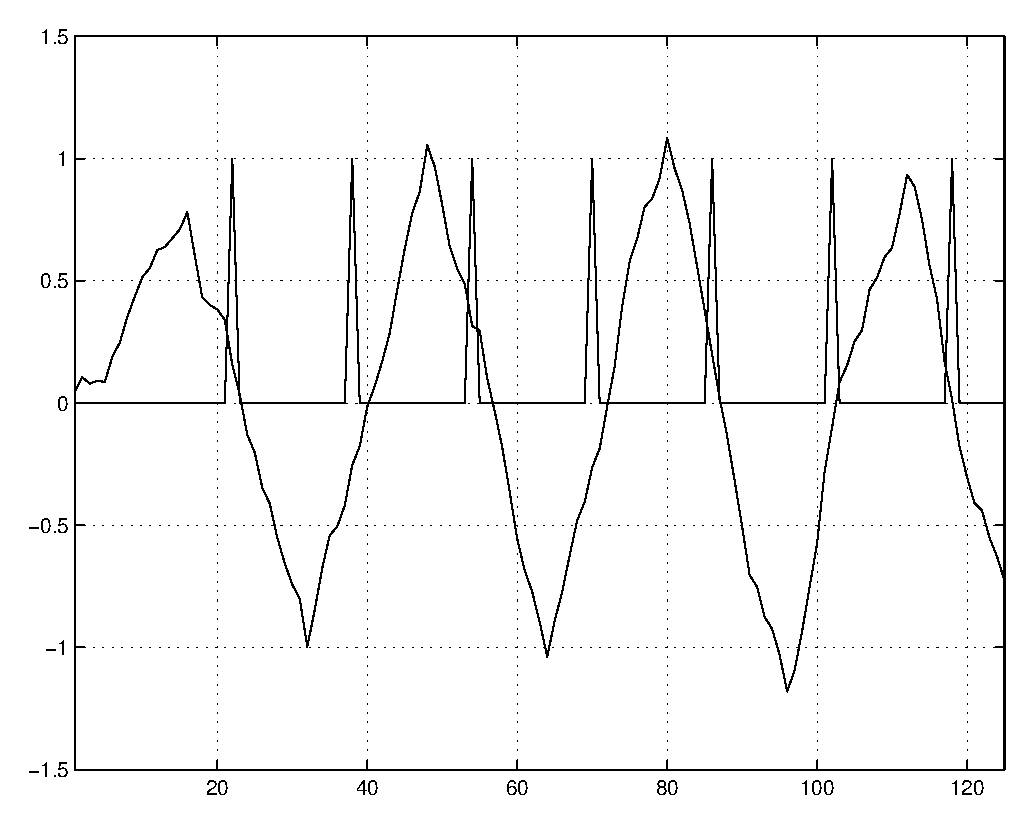
\epsfig{file=non_locked_dll.eps,width=6cm}
      \caption{Symbol sampling before DLL lock.}
      \label{fig: dll_before_lock}
   \end{center}
\end{figure}

\begin{figure}[ht]
   \begin{center}
      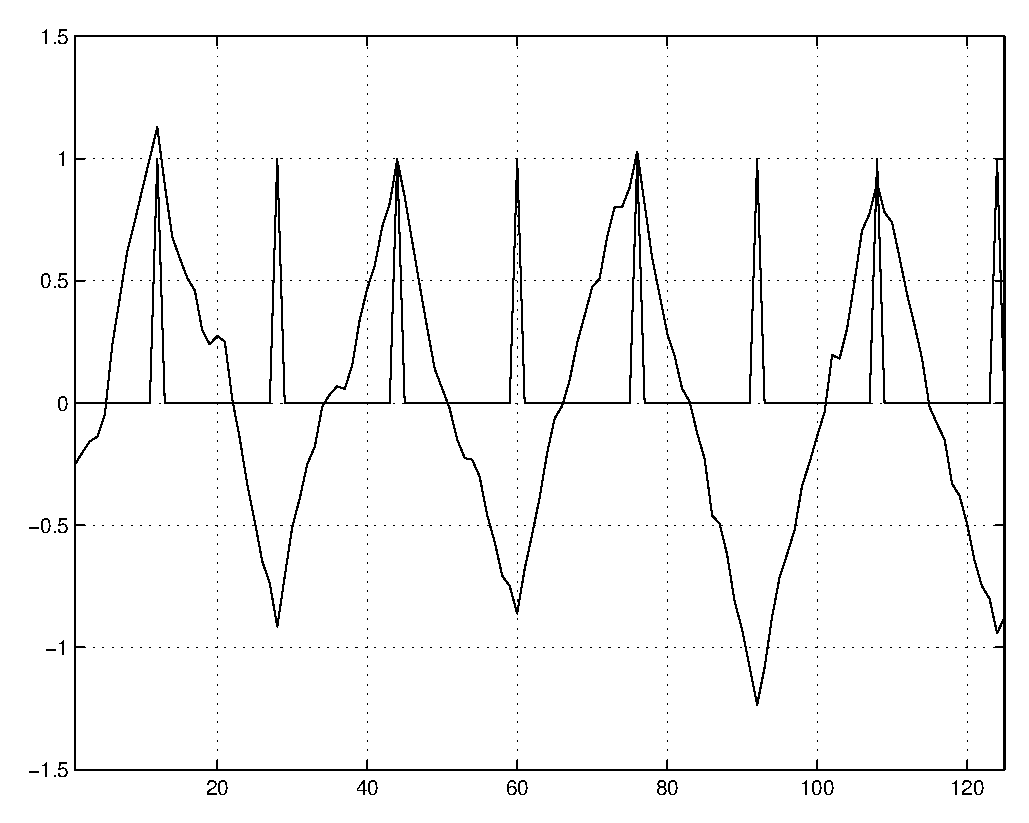
\epsfig{file=locked_dll.eps,width=6cm}
      \caption{Symbol sampling after DLL lock.}
      \label{fig: dll_after_lock}
   \end{center}
\end{figure}



\section{DSP Implementation}

Once a working \matlab simulation is completed, the DSP implementation 
of this exercise is relatively straight forward.  To test your
implementation you can use the function generator to generate
a BPSK waveform by setting it to a square wave of the correct 
frequency.  
You should send the on-time sample as well as the averaging filter output
to the D/A to verify that your system is working. 

\section{Extensions}

As your final project will require some modification to the discussed
BPSK signaling, you will want to refer to the listed references,
\cite{Proakis1, Blahut1}, and
consider some of the following questions regarding such modifications:

$\bullet$ How much noise is necessary to disrupt the symbol-timing?

$\bullet$ What happens when the input is random 
          (not simply $+1, -1, +1, -1, ...$)?

$\bullet$ What would the matched filter look like for different symbol shapes?
 
$\bullet$ What other methods of symbol timing are available for your 
          application?

$\bullet$ How does accumulating the early-late decisions help suppress the 
          effects of noise?


\bibliographystyle{ieeetr}
\bibliography{../../ece320}

\end{document}
\bye








